\documentclass[a4paper,12pt]{article}
\usepackage[activate={true,nocompatibility},final,tracking=true,kerning=true,spacing=true,factor=1100,stretch=10,shrink=10]{microtype}
\usepackage[english]{babel}
\usepackage[utf8]{inputenc}
\usepackage[nottoc]{tocbibind}
\usepackage[final]{pdfpages}
\usepackage{amsmath,apacite}
\usepackage{graphicx,wrapfig}
\usepackage{tikz,pgfplots}
\usepackage{algorithm,algpseudocode}
\usetikzlibrary{matrix,chains,positioning,decorations.pathreplacing,arrows,calc,3d}

\title{Paper Title}

\author{Joshua Gruenstein and Michael Truell}

\date{\today}

\begin{document}
\maketitle

% 100-200 words

\begin{abstract}

A robot control system was developed that could be taught tasks through reinforcement learning.  The system, nicknamed Fido, was designed to be universal regardless of the specific hardware inputs and outputs and does not need to be modified for the task at hand. In addition, Fido was built to learn with limited feedback, allowing humans to train Fido in a reasonable time frame. This was achieved through the training of artificial neural networks with a wire-fitted moving least squares interpolator following the $Q$-learning reinforcement algorithm and an action selection policy that utilizes a Boltzmann distribution of probability. Robots of different drive systems were simulated with sensors to test functionality, then a small robot using the Intel Edison compute module was constructed for physical testing.  The robot was successfully trained to do an array of tasks with limited feedback, such as \textbf{TASKS GO HERE}.

\end{abstract}

\section{Introduction}

The most prevalent control system used in mobile robotics is a procedurally programmed expert system (Biggs \& MacDonald, 2003).  Such systems use conditional logic in order to emulate a desired behavior.  However, such systems are limited in numerous respects.  First, they can only perform the specific task for which they were programmed to accomplish; the entire software must be rewritten in order to change the target task.  Second, they rely on a knowledge of the inputs and outputs to the robot (such as sensors and motor control) in order to function.  The purpose of Fido was to solve both of these problems, allowing a universal general control system for robots that can be assigned tasks ``in the field'' using reinforcement learning.  

We chose to approach this problem with artificial neural networks; function appropriators modeled after nature with the capability to take in a large number of inputs to produce an output.  Neural networks are commonly used to solve tasks that are challenging using traditional rule-based programming, making them perfect for our task.  The control system was named Fido for the name's connotations to training an intelligent organism. 

Software design goes here.

\section{Neural Networks}

\begin{figure}
	\centering
	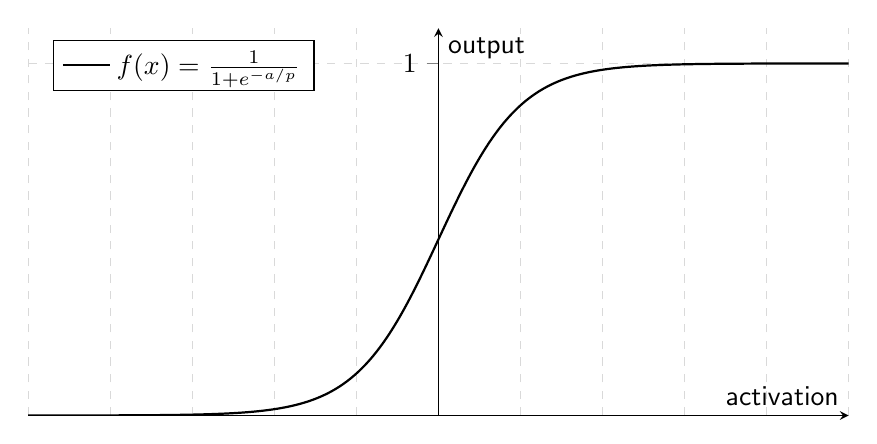
\begin{tikzpicture}[font=\sffamily]
    \begin{axis}[
    	legend pos=north west,
        axis x line=middle,
        axis y line=middle,
        grid = major,
        width=12cm,
        height=6.5cm,
        grid style={dashed, gray!30},
        xmin=-1,xmax= 1,ymin= 0,ymax= 1.1,
        xlabel=activation,ylabel=output,
        tick align=outside,
        ytick={1},
        xmajorticks=false,
        enlargelimits=false]
      \addplot[domain=-1:1,black,thick,samples=500] {1/(1+exp(-10*x))}; 
      \addlegendentry{$f(x)=\frac{1}{1+e^{-a/p}}$}
    \end{axis} 
\end{tikzpicture}
	\caption{Sigmoid Function Graph}
\end{figure}

\begin{figure}[h]
	\centering
	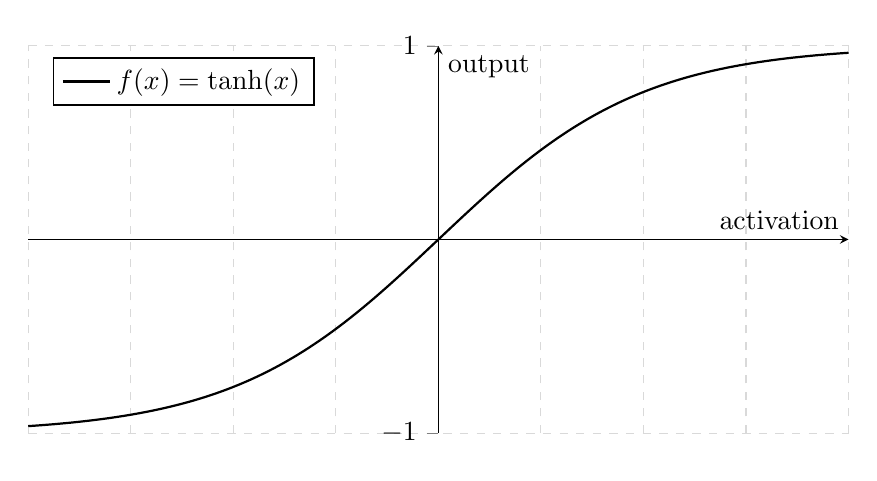
\begin{tikzpicture}
    \begin{axis}[
    	legend pos=north west,
        axis x line=middle,
        axis y line=middle,
        grid = major,
        width=12cm,
        height=6.5cm,
        grid style={dashed, gray!30},
        xmin=-2,xmax= 2,ymin= -1,ymax= 1,
        xlabel=activation,ylabel=output,
        tick align=outside,
        ytick={-1,1},
        xmajorticks=false,
        enlargelimits=false]
      \addplot[domain=-2:2,black,thick,samples=500] {tanh(x)}; 
      \addlegendentry{$f(x)=\tanh(x)$}
    \end{axis} 
\end{tikzpicture}
	\caption{Hyperbolic Tangent Function Graph}
\end{figure}

\begin{figure}[h]
	\centering
	\def\layersep{2.5cm}
\begin{tikzpicture}[shorten >=1pt,->,draw=black!50, node distance=\layersep,font=\sffamily]
    \tikzstyle{every pin edge}=[<-,shorten <=1pt]
    \tikzstyle{neuron}=[circle,line width=0.3mm,draw=black,minimum size=17pt,inner sep=0pt]
    \tikzstyle{annot} = [text width=4em, text centered]

    \foreach \name / \y in {1,...,4}
        \node[neuron, pin=left:Input \y] (I-\name) at (0,-\y) {};

    \foreach \name / \y in {1,...,5}
        \path[yshift=0.5cm]
            node[neuron] (H-\name) at (\layersep,-\y cm) {};

    \node[neuron,pin={[pin edge={->}]right:Output}, right of=H-3] (O) {};

    \foreach \source in {1,...,4}
        \foreach \dest in {1,...,5}
            \path (I-\source) edge (H-\dest);

    \foreach \source in {1,...,5}
        \path (H-\source) edge (O);

    %\draw[->] (5,-2.9) -- (5,-5) -- (1,-5) -- (1,-4.5);
    %\node (1,-4.5) {Error back propagation}

    \node[annot,above of=H-1, node distance=1cm] (hl) {Hidden layer};
    \node[annot,left of=hl] {Input layer};
    \node[annot,right of=hl] {Output layer};
\end{tikzpicture}
	\caption{Single Output Feedforward Network}
\end{figure}

%example psuedocode (http://mirrors.ibiblio.org/CTAN/macros/latex/contrib/algorithmicx/algorithmicx.pdf for reference)
\begin{algorithm}[!ht]
	\caption{FizzBuzz Algorithm}
	\begin{algorithmic}[1]
		\For{each integer $i$ 1 to 100}
			\If{$15 \mid i$}
				\State print ``FizzBuzz''
			\ElsIf{$3 \mid i$}
				\State print ``Fizz''
			\ElsIf{$5 \mid i$}
				\State print ``Buzz''
			\Else
				\State print $i$
			\EndIf
		\EndFor
	\end{algorithmic}
\end{algorithm}

\section{Reinforcement Learning}

\section{Convergent Wire Fitted Neural Network Q-Learning}


%\section{Physical Design}
%Hardware goes here.

\subsection{Input/Output Selection}

\subsection{Platform and Benchmarking}

\subsection{Final Design}

\subsection{Mechanical Implementation}

\section{Results}

Results, testing, and applications go here.

\subsection{Training Methods}

\subsection{Findings}

\subsection{Further Applications}

\section{Conclusion}

A general robotic control system nicknamed Fido was developed that learned tasks with limited feed back. Fido couple the training of artificial neural networks with a wire-fitted moving least squares interpolator to achieve a continuous state-action space $Q$-learning reinforcement algorithm implementation. Fido leveraged a Boltzmann distribution of probability based on reward to select actions, allowing it to continuously explore its state-action space. A kinematically accurate robot was simulated with a differential drive system, a sensor array, and other outputs to test Fido. The robot was trained on a number of common robotic tasks and successfully converged on these tasks in less reward iterations than all other actors tested, while maintaining impressively low latency. In the future, we hope to improve Fido's software further and are working toward the completion of Fido's hardware implementation.

\pagebreak
\section{Appendix}

\subsection{Electrical Schematic}

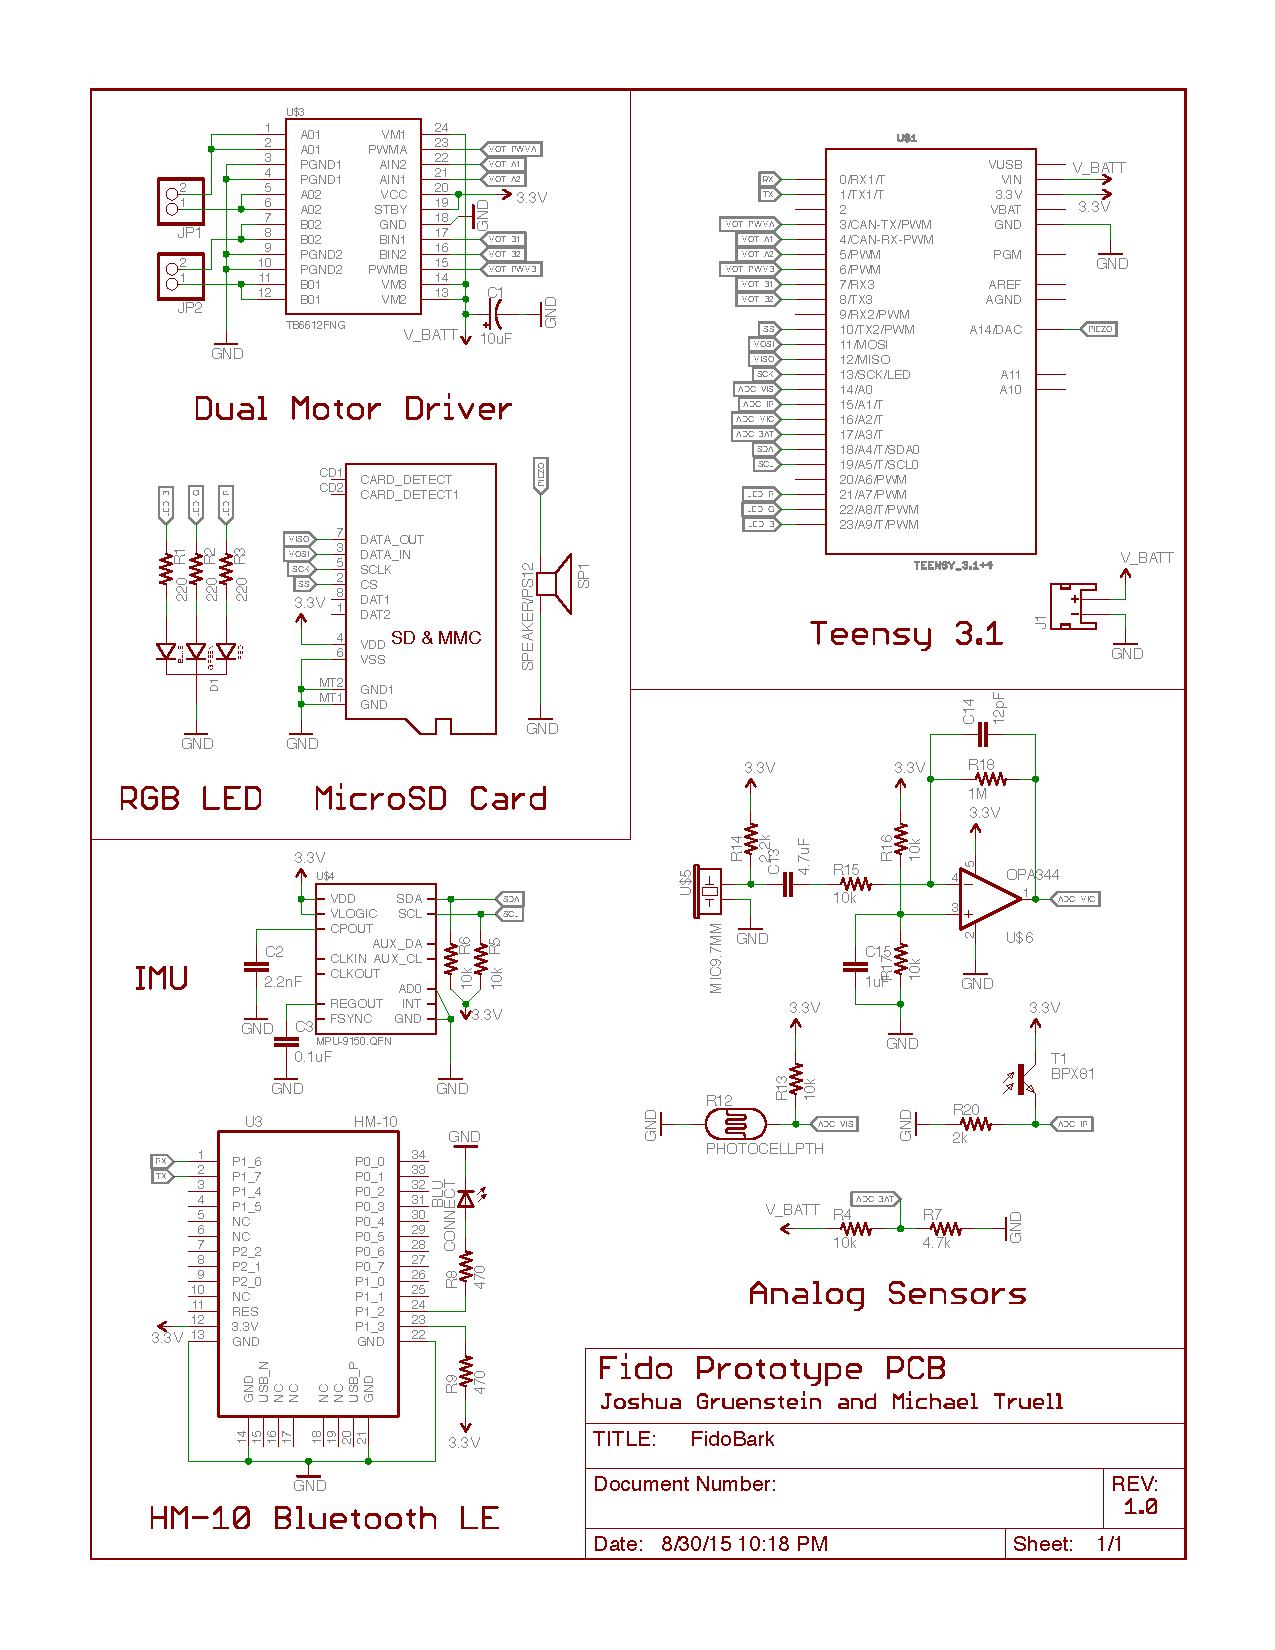
\includepdf[pages=-]{Figures/FidoBark.pdf}

\nocite{wirefit,qlearn,backprop,practical,tutorial,kinematics}

\pagebreak
\bibliography{Sections/bibliography}
\bibliographystyle{apacite}

\end{document}